\documentclass{beamer}
\usepackage[english, russian]{babel}
\usepackage[T2A]{fontenc}
\usepackage[utf8]{inputenc}
\usepackage{indentfirst}
\usepackage{amsmath, amsfonts, amssymb, amsthm, mathtools}
\usepackage[export]{adjustbox}
\usepackage{graphicx} 
\graphicspath{ {./images/} }

\usepackage{subcaption}
\usepackage{verbatim}

\usepackage{minted}{\setlength{\parskip}{0pt}}

\usepackage{hyperref}

\hypersetup{
    colorlinks=true,
    linkcolor=blue,
    filecolor=magenta,      
    urlcolor=black,
    pdftitle={Overleaf Example},
    pdfpagemode=FullScreen,
    }


\title{Лабораторная работа № 4. \\Базовая настройка HTTP-сервера Apache}
\author{Данила Стариков \\ НПИбд-02-22}
\institute{Российский университет дружбы народов имени Патриса Лумумбы}
\date{2024}

\begin{document}

\frame{\titlepage}

\begin{frame}
\frametitle{Цель работы}
\begin{itemize}
    \item Приобретение практических навыков по установке и базовому конфигурированию HTTP-сервера Apache.
\end{itemize}
\end{frame}

\begin{frame}[containsverbatim]
\frametitle{Установка HTTP-сервера}
 Установили из репозитория стандартный веб-сервер (HTTP-сервер и утилиты httpd, криптоутилиты и пр.):
\begin{minted}{bash}
LANG=C yum grouplist
dnf -y groupinstall "Basic Web Server"
\end{minted}
\end{frame}


\begin{frame}
\frametitle{Базовое конфигурирование HTTP-сервера}
    \centering
    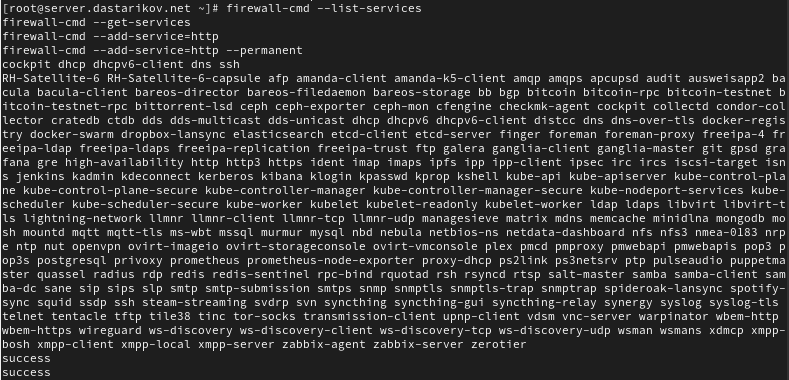
\includegraphics[width=0.9\textwidth]{../images/image01.png}
    \captionof{figure}{Настройка межсетевого экрана.}
\end{frame}

\begin{frame}
\frametitle{Базовое конфигурирование HTTP-сервера}
    \centering
    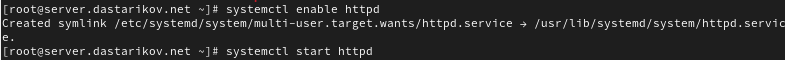
\includegraphics[width=0.9\textwidth]{../images/image02.png}
    \captionof{figure}{Запуск HTTP-сервера.}
\end{frame}

\begin{frame}
\frametitle{Анализ работы HTTP-сервера}
    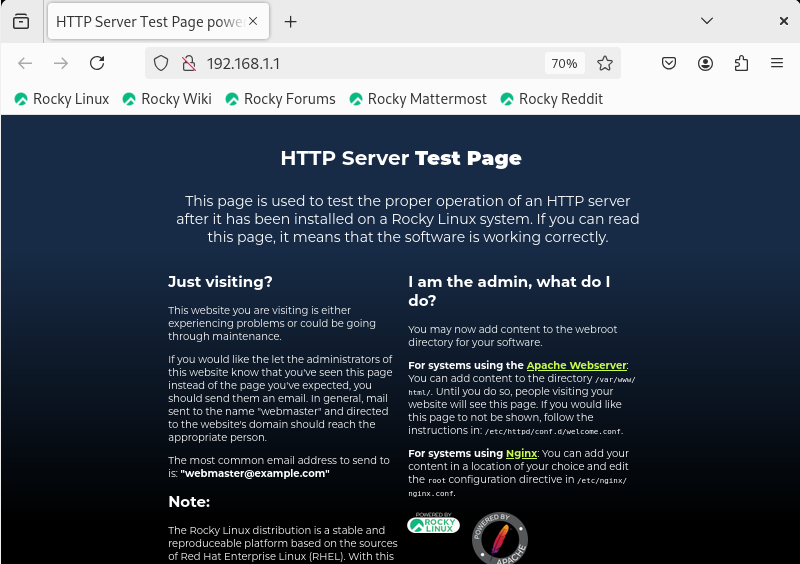
\includegraphics[width=0.9\textwidth]{../images/image03.png}
    \captionof{figure}{Запуск тестовой страницы.}
\end{frame}
 

\begin{frame}
\frametitle{Анализ работы HTTP-сервера}
    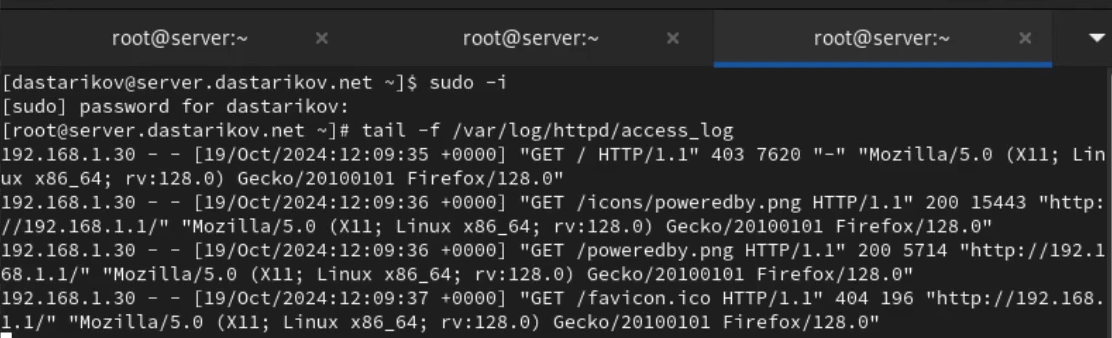
\includegraphics[width=0.9\textwidth]{../images/image14.png}
    \captionof{figure}{Записи в журнале мониторинга доступка к веб-серверу}
\end{frame}
 

\begin{frame}
\frametitle{Настройка виртуального хостинга для HTTP-сервера}
    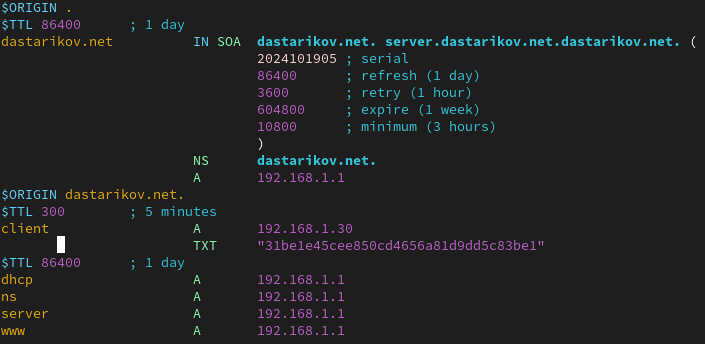
\includegraphics[width=0.9\textwidth]{../images/image05.png}
    \captionof{figure}{Обновление файла прямой DNS-зоны.}
\end{frame}
 

\begin{frame}
\frametitle{Настройка виртуального хостинга для HTTP-сервера}
    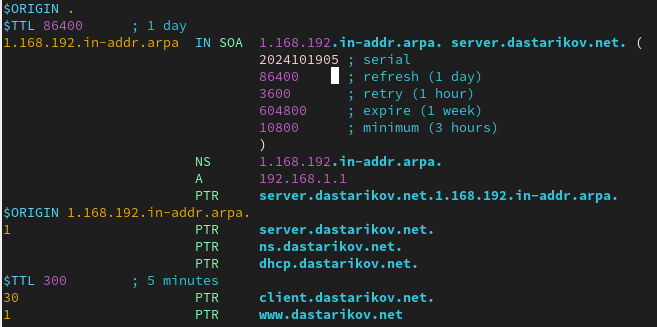
\includegraphics[width=0.9\textwidth]{../images/image07.png}
    \captionof{figure}{Обновление файла обратной DNS-зоны.}
\end{frame}

\begin{frame}
\frametitle{Настройка виртуального хостинга для HTTP-сервера}
    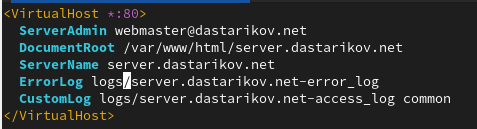
\includegraphics[width=0.9\textwidth]{../images/image08.png}
    \captionof{figure}{Изменение server.dastarikov.net.conf.}
\end{frame}

\begin{frame}
\frametitle{Настройка виртуального хостинга для HTTP-сервера}
    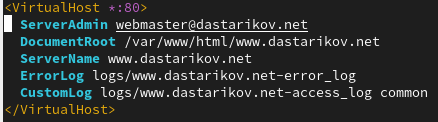
\includegraphics[width=0.9\textwidth]{../images/image09.png}
    \captionof{figure}{Изменение www.dastarikov.net.conf.}
\end{frame}

\begin{frame}
\frametitle{Настройка виртуального хостинга для HTTP-сервера}
    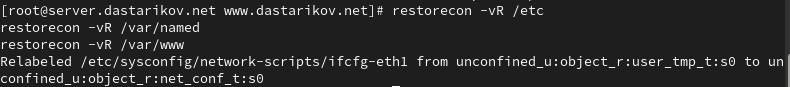
\includegraphics[width=0.9\textwidth]{../images/image10.png}
    \captionof{figure}{Восстановление контекста безопасности SELinux.}
\end{frame}

\begin{frame}
\frametitle{Настройка виртуального хостинга для HTTP-сервера}
    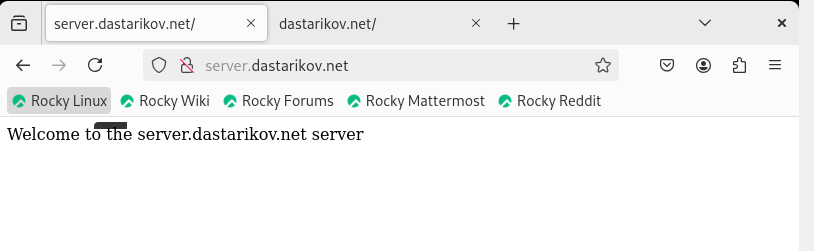
\includegraphics[width=0.9\textwidth]{../images/image11.png}
    \captionof{figure}{Проверка доступа к server.dastarikov.net.}
\end{frame}

\begin{frame}
\frametitle{Настройка виртуального хостинга для HTTP-сервера}
    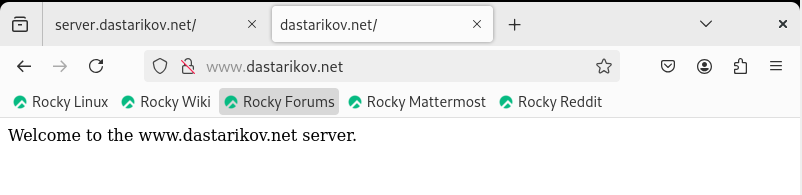
\includegraphics[width=0.9\textwidth]{../images/image12.png}
    \captionof{figure}{Проверка доступа к www.dastarikov.net.}
\end{frame}


\begin{frame}[containsverbatim]
\frametitle{Внесение изменений в настройки внутреннего окружения виртуальной машины}
Открыв его на редактирование, прописали в нём следующий скрипт:
\begin{minted}[fontsize=\small]{bash}
#!/bin/bash
echo "Provisioning script $0"
echo "Install needed packages"
dnf -y groupinstall "Basic Web Server"
echo "Copy configuration files"
cp -R /vagrant/provision/server/http/etc/httpd/* /etc/httpd
cp -R /vagrant/provision/server/http/var/www/* /var/www
chown -R apache:apache /var/www
restorecon -vR /etc
restorecon -vR /var/www
echo "Configure firewall"
firewall-cmd --add-service=http
firewall-cmd --add-service=http --permanent
echo "Start http service"
systemctl enable httpd
systemctl start httpd
\end{minted}
\end{frame}


\begin{frame}
\frametitle{Выводы}
\begin{itemize}
    \item В результате выполнения лабораторной работы получили навыки по установке и базовому конфигурированию HTTP-сервера Apache.
\end{itemize}
\end{frame}
\end{document}
